\documentclass[a4paper,10pt,twocolumn]{ltjarticle}
\usepackage{kaitoushu}

\pgfplotsset{
  myaxis/.style={
    axis lines=middle,
    xlabel={$x$}, ylabel={$y$},
    every axis x label/.style={at={(ticklabel* cs:1)},anchor=west},
    every axis y label/.style={at={(ticklabel* cs:1)},anchor=south},
    tick label style={font=\scriptsize},
    label style={font=\small},
    width=5.5cm, height=5cm,
    grid=none,
    samples=200,
  }
}

\begin{document}

\problemrange{3章：関数とグラフ — 練習問題2・B (p.100)}



\mondai{1}{$y=\dfrac{ax+b}{x+c}$ のグラフが原点を通り，漸近線が直線 $x=1$ と直線 $y=2$ であるという．定数 $a$，$b$，$c$ の値を定めよ．}
\kotae{
分子を整理：
\[
y=\dfrac{ax+b}{x+c}=a+\dfrac{b-ac}{x+c}
\]

漸近線 $x=-c=1 \Rightarrow c=-1$

漸近線 $y=a=2 \Rightarrow a=2$

原点通過：$\dfrac{0+b}{0+c}=0 \Rightarrow b=0$

$\therefore a=2,\;b=0,\;c=-1$
}

\mondai{2}{$y=\sqrt{-x}$ のグラフを $x$ 軸方向に $2$，$y$ 軸方向に $k$ 平行移動すると，原点を通る曲線になるという．定数 $k$ の値を定めよ．}
\kotae{
平行移動後：$y=\sqrt{-(x-2)}+k=\sqrt{2-x}+k$

原点 $(0,0)$ 通過：$0=\sqrt{2}+k$

$\therefore k=-\sqrt{2}$
}

\mondai{3}{関数 $y=\sqrt{2-x}$ が $a\leqq x\leqq 1$ の範囲で最大値 $3$ をとるように，定数 $a$ の値を定めよ．}
\kotae{
$y=\sqrt{2-x}$ は $x$ について単調減少．よって区間の左端 $x=a$ で最大．

$\sqrt{2-a}=3 \Rightarrow 2-a=9 \Rightarrow a=-7$

なお $a\leqq1$ を満たす．

$\therefore a=-7$
}

\mondai{4}{関数 $y=\dfrac{2x-1}{x+k}$ の逆関数が，また，$y=\dfrac{2x-1}{x+k}$ となるように定数 $k$ の値を定めよ．}
\kotae{
$y=\dfrac{2x-1}{x+k}$ を $x$ について解く：
\[
y(x+k)=2x-1 \Rightarrow x(y-2)=-1-ky
\]
\[
x=\dfrac{-1-ky}{y-2}=\dfrac{ky+1}{2-y}
\]

よって逆関数は $y=\dfrac{kx+1}{2-x}$．

これが元の式と等しい条件：
\[
\dfrac{kx+1}{2-x}=\dfrac{2x-1}{x+k}
\]

分母払い：$(kx+1)(x+k)=(2x-1)(2-x)$

左辺 $=kx^{2}+(k^{2}+1)x+k$

右辺 $=-2x^{2}+5x-2$

係数比較：$k=-2$，$k^{2}+1=5$（$k=\pm2$），$k=-2$

$\therefore k=-2$
}

\mondai{5}{関数 $f(x)=\dfrac{ax+b}{x-2}$ について，$y=f(x)$ の逆関数を $y=g(x)$ とする．$f(1)=2$，$g(4)=3$ であるとき，定数 $a$，$b$ の値を定めよ．}
\kotae{
$g(4)=3 \Leftrightarrow f(3)=4$．

$f(1)=2$：$\dfrac{a+b}{1-2}=2 \Rightarrow a+b=-2\;\cdots$①

$f(3)=4$：$\dfrac{3a+b}{3-2}=4 \Rightarrow 3a+b=4\;\cdots$②

②$-$①：$2a=6 \Rightarrow a=3$，$b=-5$

$\therefore a=3,\;b=-5$
}

\mondai{6}{次の問いに答えよ．}
\kotae{
\textbf{(1)} $y=\dfrac{2x+1}{x+2}=2-\dfrac{3}{x+2}$\quad 漸近線 $x=-2,\;y=2$．

$y=2-x$\quad 直線．

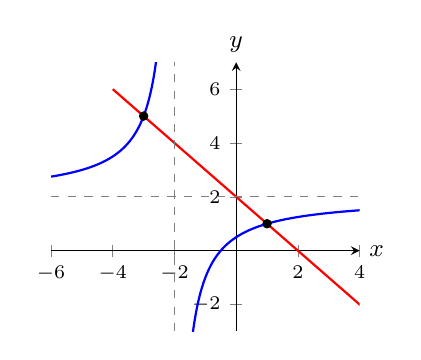
\begin{tikzpicture}
\begin{axis}[myaxis, xmin=-6,xmax=4,ymin=-3,ymax=7]
\addplot[thick,blue,domain=-6:-2.3]{(2*x+1)/(x+2)};
\addplot[thick,blue,domain=-1.7:4]{(2*x+1)/(x+2)};
\addplot[thick,red,domain=-4:5]{2-x};
\addplot[dashed,gray] coordinates {(-2,-3)(-2,7)};
\addplot[dashed,gray] coordinates {(-6,2)(4,2)};
\addplot[only marks,mark=*,mark size=1.5pt] coordinates {(-3,5)(1,1)};
\end{axis}
\end{tikzpicture}

\textbf{(2)} 交点：$\dfrac{2x+1}{x+2}=2-x$

両辺に $x+2$ をかけて $2x+1=(2-x)(x+2)=4-x^{2}$
\[
x^{2}+2x-3=0 \Rightarrow (x+3)(x-1)=0
\]
$x=-3,\;1$．対応する $y$ は $5,\;1$．

交点：$(-3,5),\;(1,1)$

\textbf{(3)} $\dfrac{2x+1}{x+2}<2-x$

移項して通分：
\[
\dfrac{2x+1-(2-x)(x+2)}{x+2}<0
\]
\[
\dfrac{x^{2}+2x-3}{x+2}<0 \Rightarrow \dfrac{(x+3)(x-1)}{x+2}<0
\]

符号表で $x=-3,\;-2,\;1$ を区切って考える：

$\therefore x<-3$ または $-2<x<1$
}

\mondai{7}{グラフを利用して，次の不等式を解け．}
\kotae{
\textbf{(1)} $\sqrt{x+6}>x$

真数条件：$x\geqq-6$．$\sqrt{x+6}\geqq0$ なので $x<0$ のときは常に成立．

$x\geqq0$ では両辺2乗して $x+6>x^{2}$，すなわち $x^{2}-x-6<0$．

$(x-3)(x+2)<0 \Rightarrow -2<x<3$

$x\geqq0$ と合わせて $0\leqq x<3$．

$x<0$ と合わせて $-6\leqq x<3$

$\therefore -6\leqq x<3$

\textbf{(2)} $\dfrac{2}{x-1}>x$

\textbf{(i) $x>1$}：両辺に正の $x-1$ をかけて
$2>x(x-1) \Rightarrow x^{2}-x-2<0 \Rightarrow (x-2)(x+1)<0$
$\Rightarrow -1<x<2$．$x>1$ と合わせて $1<x<2$．

\textbf{(ii) $x<1$}：両辺に負の $x-1$ をかけると不等号反転
$2<x(x-1) \Rightarrow x^{2}-x-2>0 \Rightarrow x<-1$ または $x>2$
$x<1$ と合わせて $x<-1$．

$\therefore x<-1$ または $1<x<2$
}

\end{document}
